\documentclass[11pt,a4paper]{article}
\usepackage[T1]{fontenc}
\usepackage[margin=2.3cm]{geometry}
\usepackage{amsmath,amssymb}
\usepackage{graphicx}
\usepackage[dvipsnames]{xcolor}
\usepackage{enumitem}
\usepackage[colorlinks=true,linkcolor=blue,urlcolor=blue]{hyperref}
\setlength{\parskip}{0.6em}
\setlength{\parindent}{0pt}
\begin{document}

\begin{center}{\LARGE\bfseries openbreakeven}\\[0.4em]{\large Find the break-even point of a small business, in five sessions.}\\[0.2em]\small PAN IIT OSS explainer \textbullet{} secondary school to diploma / undergraduate (levels 3-5)\end{center}

\section*{Why this exists}
Every small business pays some costs whether or not it sells anything, and earns a little on each sale. This explainer shows how to find the sales at which income catches up with cost, how safe that point is, and how uncertainty and time change the answer, using only straight lines, a little algebra and a random-number simulation.

\section*{The end goal}
Find the break-even point of a small business. The end goal is to find the break-even point of a small business, and to know how far to trust it. The same ideas appear in pricing, planning a start-up and any decision where a fixed cost must be recovered. All examples are made up and this is general education, not financial advice.

\section*{How the five sessions build up}
\begin{enumerate}[nosep]
\item \textbf{Session 1: Where does income catch up with cost?} (Level 1, conceptual interactive model, 60 min).
\item \textbf{Session 2: The break-even equations: contribution, safety and leverage} (Level 2, mathematical engineering model, 75 min).
\item \textbf{Session 3: Break-even under mix, steps, uncertainty and time} (Level 3, simulation and validation, 90 min).
\item \textbf{Session 4: When price and demand move together} (Level 3, simulation and validation, 90 min).
\item \textbf{Session 5: Seasons and a loan} (Level 3, simulation and validation, 90 min).
\end{enumerate}

\section{Session 1: Where does income catch up with cost?}

\subsection*{A. Real-world problem}
You want to run a lemonade stall. Before you sell a single cup you must pay 60 dollars for the stall, a pitcher and a sign. After that each cup costs 50 cents to make and sells for 2 dollars. At the start you are 60 dollars behind. How many cups until your total income has caught up with your total cost? That number is the break-even point. (General education only: the stall is made up and this is not financial advice.)

\subsection*{B. Concept and theory}
The fixed cost F is paid once, however many cups you sell. The variable cost v is paid for every cup. So the total cost after q cups is F + v q, a straight line that starts at F. The income is the price p times q, a straight line that starts at 0. Profit is income minus cost. Each cup earns p - v dollars towards paying off F, so the cups needed are F divided by what one cup earns. If p is not larger than v, a cup earns nothing and income never catches up: there is no break-even.

\begin{itemize}[nosep]
\item F: fixed cost, paid once (dollars)
\item v: variable cost of one cup (dollars per cup)
\item p: price of one cup (dollars per cup)
\item q: cups sold (cups)
\item q*: break-even number of cups (cups)
\end{itemize}

\begin{equation*}
\text{cost}(q)=F+v\,q,\qquad \text{income}(q)=p\,q
\end{equation*}

\begin{equation*}
\text{profit}(q)=p\,q-(F+v\,q)=(p-v)\,q-F
\end{equation*}

\begin{equation*}
q^{*}=\frac{F}{p-v}\quad(\text{only if } p>v)
\end{equation*}

\begin{center}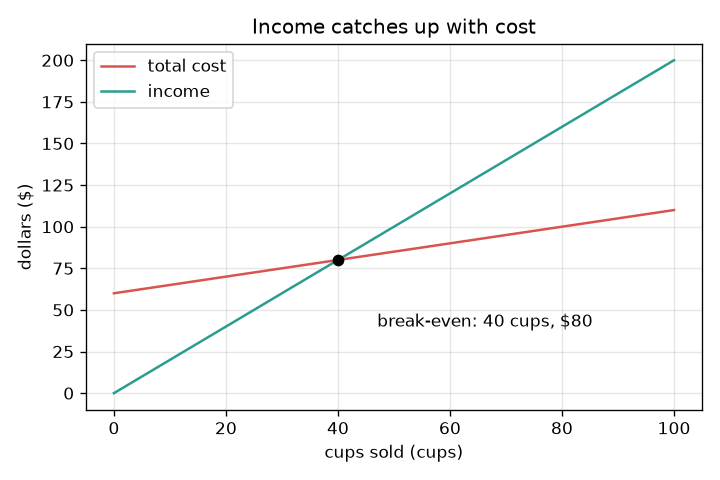
\includegraphics[width=0.85\linewidth]{figures/s01_stall_lines.png}\\\small Cost and income against cups sold: they cross at 40 cups and 80 dollars.\end{center}

\subsection*{E. Worked example}
A stall has fixed cost 60 dollars, sells cups at 2.00 dollars and spends 0.50 dollars per cup. Find the break-even number of cups and check it.
\begin{enumerate}[nosep]
\item Each cup earns 2.00 - 0.50 = 1.50 dollars towards the fixed cost.
\item Cups needed = 60 / 1.50 = 40 cups.
\item Check cost: 60 + 0.50 * 40 = 80 dollars. Check income: 2.00 * 40 = 80 dollars. They are equal.
\item One cup earlier, at 39 cups, the profit is minus 1.50 dollars; one cup later, at 41 cups, it is plus 1.50 dollars.
\end{enumerate}
\textbf{Answer.} Break-even is at 40 cups, where income and cost are both 80 dollars.

\subsection*{F. Questions}
\begin{enumerate}[nosep]
\item \textbf{Conceptual.} A friend says: the stall costs 60 dollars and each cup sells for 2 dollars, so break-even is 60 / 2 = 30 cups. What did they forget?
\item \textbf{Numerical.} A different stall has fixed cost 45 dollars, price 1.50 dollars and a cup cost of 0.60 dollars. Find the break-even cups and check that income equals cost there.
\item \textbf{Graph and simulation interpretation.} On the graph of the first stall, read the cost, the income and the profit at 25 cups. Is the stall ahead or behind?
\item \textbf{Design and optimisation challenge.} Design: the stall will only be open for a short day. Change either the price or the fixed cost so that break-even is at 30 cups or fewer. Which would you pick and what is the risk?
\end{enumerate}

\section{Session 2: The break-even equations: contribution, safety and leverage}

\subsection*{A. Real-world problem}
A made-up neighbourhood bakery sells loaves. Each month it pays 1200 dollars for rent, an oven lease and wages, whether or not anyone buys bread. Each loaf sells for 3.50 dollars and costs 1.40 dollars in flour and energy. The owner expects to sell 800 loaves a month. How many loaves are needed to break even? How far can sales fall before the bakery loses money? How many loaves earn 600 dollars? And how risky is this business compared with another one? (General education only: the bakery and its numbers are made up and this is not financial advice.)

\subsection*{B. Concept and theory}
Profit = income - cost = p q - (F + v q) = (p - v) q - F. The contribution margin p - v is what each loaf contributes towards the fixed cost; its share of the price, (p - v) / p, is the contribution ratio. Setting profit to zero gives the break-even quantity q* = F / (p - v), and the break-even revenue is p q*, which equals F divided by the contribution ratio. The margin of safety, (q - q*) / q, is the share by which sales can fall before the profit disappears. For a target profit T, the quantity is (F + T) / (p - v). The degree of operating leverage, DOL = (p - v) q / profit, tells how strongly profit reacts to sales: a 10 percent change in sales changes profit by DOL times 10 percent. A business with big fixed costs has a high DOL: it gains a lot in good months and loses a lot in bad ones. For the design problem the quantity depends on the price through an estimated demand line, q = a - b p, so profit is a quadratic in p.

\begin{itemize}[nosep]
\item p: price per loaf (dollars per loaf)
\item v: variable cost per loaf (dollars per loaf)
\item F: fixed cost per month (dollars per month)
\item q: loaves sold per month (loaves per month)
\item q*: break-even quantity (loaves per month)
\item T: target profit (dollars per month)
\item a, b: demand line: a = 1675 loaves, b = 250 loaves per dollar (loaves; loaves per dollar)
\item DOL: degree of operating leverage (no unit)
\end{itemize}

\begin{equation*}
\text{profit}=(p-v)\,q-F
\end{equation*}

\begin{equation*}
q^{*}=\frac{F}{p-v},\qquad \text{break-even revenue}=p\,q^{*}=\frac{F}{1-v/p}
\end{equation*}

\begin{equation*}
\text{margin of safety}=\frac{q-q^{*}}{q},\qquad q_T=\frac{F+T}{p-v}
\end{equation*}

\begin{equation*}
\mathrm{DOL}=\frac{(p-v)\,q}{\text{profit}}=\frac{\%\text{ change in profit}}{\%\text{ change in sales}}
\end{equation*}

\begin{equation*}
(p-v)(a-b\,p)-F=T\;\Longrightarrow\; b\,p^{2}-(a+b\,v)\,p+(a\,v+F+T)=0
\end{equation*}

\begin{center}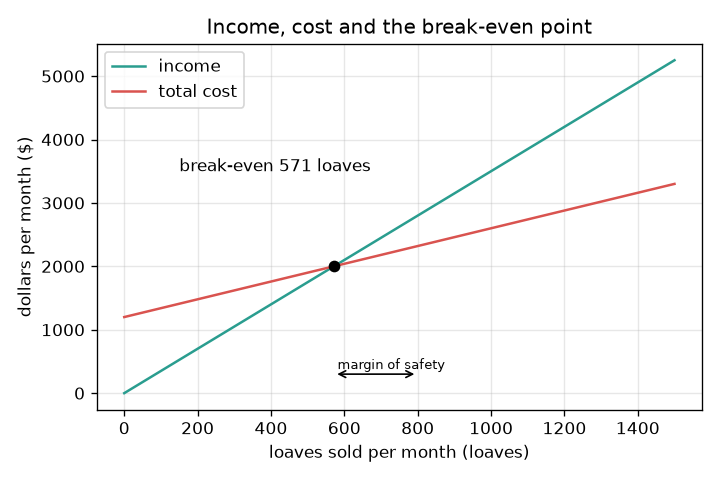
\includegraphics[width=0.85\linewidth]{figures/s02_cvp_lines.png}\\\small Income and cost against loaves: break-even at 571 loaves and the margin of safety up to 800.\end{center}

\subsection*{E. Worked example}
For F = 1200 dollars, p = 3.50, v = 1.40 and 800 loaves a month, find the break-even quantity and revenue, the profit, the margin of safety, the loaves needed for a 600 dollar profit and the DOL. Then test the DOL with a 10 percent change in sales.
\begin{enumerate}[nosep]
\item Contribution margin = 3.50 - 1.40 = 2.10 dollars per loaf; contribution ratio = 2.10 / 3.50 = 0.60.
\item Break-even quantity = 1200 / 2.10 = 571.43 loaves, so 572 whole loaves. Break-even revenue = 1200 / 0.60 = 2000 dollars.
\item Profit at 800 loaves = 2.10 * 800 - 1200 = 480 dollars.
\item Margin of safety = (800 - 571.43) / 800 = 0.2857, about 28.6 percent.
\item Loaves for 600 dollars: (1200 + 600) / 2.10 = 857.14, so 858 whole loaves.
\item DOL = 2.10 * 800 / 480 = 3.5. Test: sales up 10 percent (880 loaves) give profit 648 dollars, which is 35 percent more; sales down 10 percent (720 loaves) give 312 dollars, 35 percent less.
\item Scanning q on a fine grid and stopping when profit reaches zero also finds 571.43, so the formula is right.
\end{enumerate}
\textbf{Answer.} Break-even 571.43 loaves (572 whole) or 2000 dollars; profit 480 dollars at 800 loaves; margin of safety 28.6 percent; 858 loaves for 600 dollars; DOL 3.5, so a 10 percent change in sales moves profit by 35 percent.

\subsection*{F. Questions}
\begin{enumerate}[nosep]
\item \textbf{Conceptual.} Two bakeries both earn 480 dollars at 800 loaves. Bakery X is the one in the worked example. Bakery Y has fixed cost 600 dollars and a variable cost of 2.15 dollars per loaf (more hired help, less rent), both at price 3.50. Which is riskier if sales fall by 10 percent, and why?
\item \textbf{Numerical.} A cafe has F = 900 dollars, price 5 dollars and variable cost 2 dollars. Find the break-even quantity and revenue, and the quantity needed for a 600 dollar profit. Check the units.
\item \textbf{Graph and simulation interpretation.} On the profit-against-loaves line of the worked example, what are the value at 0 loaves, the slope, and the point where it crosses zero? What does each mean?
\item \textbf{Design and optimisation challenge.} Design: with demand q = 1675 - 250 p, variable cost 1.40 dollars and fixed cost 1200 dollars, choose a price that gives 500 dollars profit. How many prices work, what do they sell, and can the bakery reach 600 dollars?
\end{enumerate}

\section{Session 3: Break-even under mix, steps, uncertainty and time}

\subsection*{A. Real-world problem}
The made-up bakery of Session 2 is more complicated than one loaf at one price. It also sells cakes. When it grows it needs a second oven. Its price, its flour cost and its customers are never exactly what the plan says. And the start-up money is paid back slowly, month by month. A single break-even number hides all of that. Can we build a richer model, check it against a formula, and decide which input to watch and which price and oven size to choose? (General education only: made-up numbers, not financial advice.)

\subsection*{B. Concept and theory}
Several products: the sales mix gives each product's share of the units sold; the weighted contribution margin is the mix-weighted average of (p - v), and the break-even units of the whole business are F divided by it. A different mix gives a different break-even, even with the same fixed cost. Step-fixed costs: if one oven bakes at most 700 loaves a month and a second oven adds a fixed cost above that, the fixed cost jumps and so does the profit line, so profit can cross zero several times; we find the crossings by scanning whole loaves and compare them with F\_k / (p - v) for each oven count k. Uncertainty: we draw 20000 random months with a fixed seed from normal distributions for price, variable cost and demand, compute the profit of each and count how many are negative. Reference: if only demand is random, the loss probability is the normal probability that demand is below q*. Sensitivity: change one input by minus and plus 10 percent and note the profit; the input with the widest swing matters most (a tornado chart). Time value: money received later is worth less. Discounting divides month t's cash by (1 + r)\textasciicircum{}t, with monthly rate r = (1 + annual rate)\textasciicircum{}(1/12) - 1. Payback is the first month the running total reaches the start-up cost; NPV is the discounted cash minus the start-up cost. Failure cases: if p \textless{}= v there is no break-even; if demand falls as price rises there are up to two break-even prices, or none if the fixed cost is too big.

\begin{itemize}[nosep]
\item w: weighted contribution margin (dollars per unit)
\item s\_i: share of units for product i (no unit)
\item k: number of ovens (no unit)
\item cap: loaves one oven can bake (700) (loaves per month)
\item sigma: standard deviation of a random input (same as the input)
\item r: monthly discount rate (per month)
\item NPV: net present value (dollars)
\item C0: start-up cost (dollars)
\end{itemize}

\begin{equation*}
w=\sum_i s_i\,(p_i-v_i),\qquad q^{*}_{\text{units}}=\frac{F}{w}
\end{equation*}

\begin{equation*}
F_k=F_1+(k-1)\,\Delta F,\qquad q_k=\frac{F_k}{p-v}\ \text{valid if}\ (k-1)\,\mathrm{cap}<q_k\le k\,\mathrm{cap}
\end{equation*}

\begin{equation*}
\text{profit}=(p-v)\,q-F,\quad p\sim N(\mu_p,\sigma_p^{2}),\ v\sim N(\mu_v,\sigma_v^{2}),\ q\sim N(\mu_q,\sigma_q^{2})
\end{equation*}

\begin{equation*}
P(\text{loss})=\Phi\!\left(\frac{q^{*}-\mu_q}{\sigma_q}\right)\quad(\text{only demand random})
\end{equation*}

\begin{equation*}
r=(1+i)^{1/12}-1,\qquad \mathrm{NPV}=-C_0+\sum_{t=1}^{n}\frac{c_t}{(1+r)^{t}}
\end{equation*}

\begin{equation*}
(p-v)(a-b\,p)=F\;\Longrightarrow\;b\,p^{2}-(a+b\,v)\,p+(a\,v+F)=0\ \ (\text{no real root: no break-even})
\end{equation*}

\begin{center}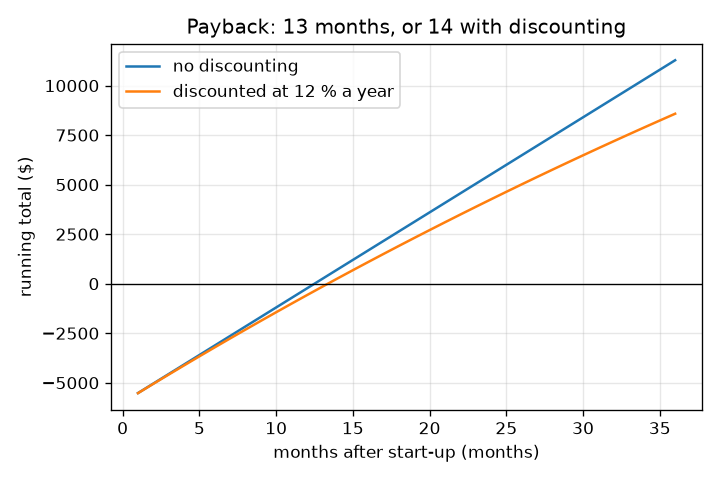
\includegraphics[width=0.85\linewidth]{figures/s03_payback.png}\\\small Running cash total after a 6000 dollar start-up: payback at month 13, month 14 when discounted.\end{center}

\subsection*{E. Worked example}
The bakery sells loaves (price 3.50, variable cost 1.40) and cakes (price 18, variable cost 9) in the unit mix 80 percent loaves and 20 percent cakes, with F = 1200 dollars. Find the break-even, then find the profit crossings if a second oven (900 dollars more) is needed above 700 loaves, and the chance of a loss when only demand is random (mean 800, standard deviation 150, loaves only).
\begin{enumerate}[nosep]
\item Weighted margin = 0.8 * 2.10 + 0.2 * 9.00 = 1.68 + 1.80 = 3.48 dollars per unit.
\item Break-even units = 1200 / 3.48 = 344.8, which is about 275.9 loaves and 69.0 cakes. If the mix shifts to 90 percent loaves the weighted margin is 2.79 and the break-even rises to 430.1 units; at 60 percent loaves it is 246.9 units.
\item Step costs, loaves only: with one oven (fixed 1200) the break-even is 571.43 loaves; profit at 700 loaves is 270 dollars. At 701 loaves the fixed cost is 2100 and the profit is minus 627.90 dollars. With two ovens the break-even is 2100 / 2.10 = 1000 loaves. Scanning whole loaves finds the sign changes at 572 (up), 701 (down) and 1000 (up).
\item Loss chance with only demand random: q* = 571.43, so z = (571.43 - 800) / 150 = -1.524 and P(loss) = 0.0638, about 6.4 percent. The simulation of 20000 months gives about 6.5 percent.
\end{enumerate}
\textbf{Answer.} Break-even 344.8 units for the 80/20 mix (275.9 loaves, 69.0 cakes); with the second oven the profit crosses zero up at 572, down at 701 and up again at 1000 loaves; the loss chance with only demand random is about 6.4 percent by formula and 6.5 percent by simulation.

\subsection*{F. Questions}
\begin{enumerate}[nosep]
\item \textbf{Conceptual.} Why can the break-even of a two-product business go down even though the fixed cost and all prices stay the same?
\item \textbf{Numerical.} A 6000 dollar oven and fit-out earns 480 dollars of cash each month. Find the simple payback month, the discounted payback month at 12 percent a year, and the NPV over 24 months at that rate.
\item \textbf{Graph and simulation interpretation.} In the Monte Carlo histogram, which part of the picture is the loss probability, and what would happen to it if demand became more uncertain (a larger standard deviation) with the same mean?
\item \textbf{Design and optimisation challenge.} Design: the owner may choose the 600, 800 or 1000 loaf oven and a price from 3.00 to 5.00 dollars in 0.25 steps. A choice passes if the loss probability is at most 5 percent, the payback at most 12 months and the margin of safety at least 20 percent. Use \texttt{evaluate} to recommend one choice and explain the trade-off.
\end{enumerate}

\section{Session 4: When price and demand move together}

\subsection*{A. Real-world problem}
In Session 3 the made-up bakery's price, variable cost and demand were random but independent: a higher price than planned said nothing about demand. Real customers are not like that. When the price is above plan, fewer people buy; in a festival week a higher price can even come with more buyers. With the same averages and the same spreads, how much does this link change the chance that a month makes a loss? And which link should a lender believe? (Made-up bakery and numbers; general education only, not financial advice.)

\subsection*{B. Concept and theory}
The correlation rho of two random numbers is a number from -1 to +1. At -1 a high price always comes with low demand, at 0 there is no linear link and at +1 they always rise together. To draw demand with correlation rho to the price we mix two independent standard normal draws, z\_p for the price and z\_o for everything else: z\_d = rho z\_p + sqrt(1 - rho\textasciicircum{}2) z\_o, and then demand = mean + sd z\_d. The price and the variable cost are drawn exactly as in Session 3, so rho = 0 reproduces Session 3 to the last digit.

Write profit = X D - F, where X = price - variable cost and D = demand. X and D are jointly normal, so the mean and the standard deviation of X D have exact formulas (Isserlis' theorem). With Cov(X, D) = rho sigma\_p sigma\_D (the cost is independent of both), the mean is mu\_X mu\_D + Cov - F, and the variance is mu\_X\textasciicircum{}2 sigma\_D\textasciicircum{}2 + mu\_D\textasciicircum{}2 sigma\_X\textasciicircum{}2 + 2 mu\_X mu\_D Cov + sigma\_X\textasciicircum{}2 sigma\_D\textasciicircum{}2 + Cov\textasciicircum{}2, with sigma\_X\textasciicircum{}2 = sigma\_p\textasciicircum{}2 + sigma\_v\textasciicircum{}2. The correlation moves the mean by only rho sigma\_p sigma\_D, which is 30 dollars per unit of rho here, but it moves the variance a lot.

Why? A higher price earns more on each loaf but sells fewer loaves. With rho \textless{} 0 the two effects partly cancel (a \textbf{natural hedge}) and the profit varies less. With rho \textgreater{} 0 they add and the profit varies more. The risk of a loss month therefore depends on the links between the inputs, not only on the spread of each input.

Which correlation is believable? Session 2 gave the demand line: each extra dollar of price loses 250 loaves a month. If the price wobbles by 0.20 dollars and demand follows that line, demand moves by 250 x 0.20 = 50 loaves, while the whole demand spread is 150 loaves, so the correlation is -50 / 150 = -0.33.

\begin{itemize}[nosep]
\item rho: correlation between price and demand (no unit)
\item p, v, D: price, variable cost, demand (dollars per loaf, dollars per loaf, loaves per month)
\item X: price minus variable cost (dollars per loaf)
\item sigma\_p, sigma\_v, sigma\_D: standard deviations (0.20, 0.15, 150) (dollars per loaf, dollars per loaf, loaves per month)
\item Cov: covariance of price and demand, rho sigma\_p sigma\_D (dollars x loaves per month)
\item F: fixed cost (dollars per month)
\end{itemize}

\begin{equation*}
z_d=\rho\,z_p+\sqrt{1-\rho^{2}}\,z_o,\qquad D=\mu_D+\sigma_D z_d
\end{equation*}

\begin{equation*}
E[\text{profit}]=\mu_X\mu_D+\rho\,\sigma_p\sigma_D-F
\end{equation*}

\begin{equation*}
\mathrm{Var}[X D]=\mu_X^{2}\sigma_D^{2}+\mu_D^{2}\sigma_X^{2}+2\mu_X\mu_D\,\mathrm{Cov}+\sigma_X^{2}\sigma_D^{2}+\mathrm{Cov}^{2},\qquad \mathrm{Cov}=\rho\,\sigma_p\sigma_D
\end{equation*}

\begin{equation*}
\rho_{\text{implied}}=-\frac{b\,\sigma_p}{\sigma_D}=-\frac{250\times 0.20}{150}=-0.33
\end{equation*}

\begin{center}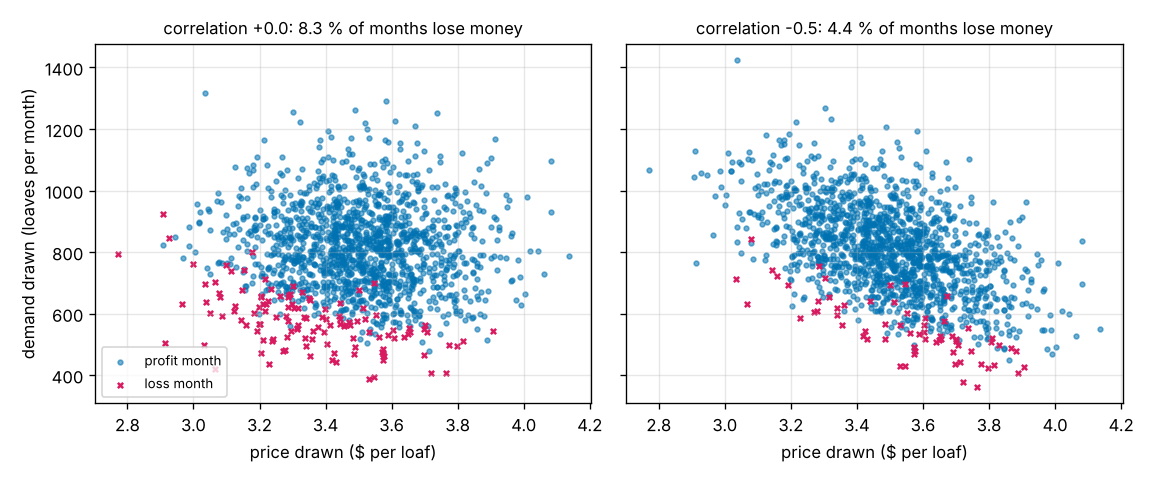
\includegraphics[width=0.95\linewidth]{figures/s04_price_demand_scatter.png}\\\small Price against demand for 1500 simulated months at correlation 0 and -0.5; the loss months are marked.\end{center}

\begin{center}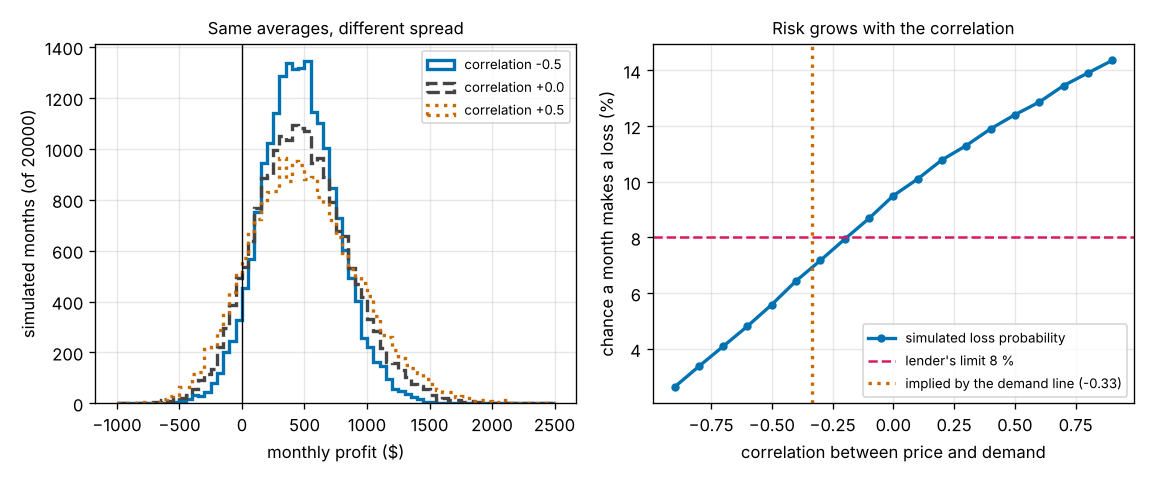
\includegraphics[width=0.95\linewidth]{figures/s04_loss_vs_rho.png}\\\small Left: profit histograms for correlation -0.5, 0 and +0.5. Right: the loss probability against the correlation.\end{center}

\subsection*{E. Worked example}
The bakery sells loaves at 3.50 dollars (variable cost 1.40), with F = 1200 dollars a month, a price wobble of 0.20, a cost wobble of 0.15 and demand of 800 loaves with sd 150. Find the mean and the standard deviation of monthly profit for correlation -0.5, estimate the loss probability from them, and compare with the simulation.
\begin{enumerate}[nosep]
\item mu\_X = 3.50 - 1.40 = 2.10, so the planned profit is 2.10 x 800 - 1200 = 480 dollars. Cov = -0.5 x 0.20 x 150 = -15.
\item Mean = 480 - 15 = 465 dollars: the correlation moved the mean by only 15 dollars.
\item sigma\_X\textasciicircum{}2 = 0.20\textasciicircum{}2 + 0.15\textasciicircum{}2 = 0.0625. Variance = 2.1\textasciicircum{}2 x 150\textasciicircum{}2 + 800\textasciicircum{}2 x 0.0625 + 2 x 2.1 x 800 x (-15) + 0.0625 x 150\textasciicircum{}2 + 15\textasciicircum{}2 = 99 225 + 40 000 - 50 400 + 1 406 + 225 = 90 456, so the standard deviation is 300.8 dollars (374.9 for independent inputs).
\item A quick estimate treats the profit as normal: z = -465 / 300.8 = -1.546 and P(loss) = 0.061 (6.1 percent). The simulation of 20000 months gives 5.6 percent, with mean 461 and standard deviation 300.
\item The normal shortcut is a little high because a product of normals is skewed: it has a longer tail on the profit side than on the loss side. For independent inputs the same shortcut gives 10.0 percent against 9.5 percent simulated.
\end{enumerate}
\textbf{Answer.} With correlation -0.5 the mean profit is 465 dollars and the standard deviation is 300.8 dollars (against 480 and 375 for independent inputs). The loss chance is about 6.1 percent by the normal shortcut and 5.6 percent by simulation, against 9.5 percent for independent inputs: a 3.9 point drop from a link that changes the mean by only 15 dollars.

\subsection*{F. Questions}
\begin{enumerate}[nosep]
\item \textbf{Conceptual.} Why does a negative correlation between price and demand make the bakery's profit less risky, although it hardly changes the average profit?
\item \textbf{Numerical.} Find the mean and the standard deviation of monthly profit for correlation +0.5 by hand (same data as the worked example), and use them to estimate the loss probability with the normal shortcut. How does it compare with the 12.4 percent of the simulation?
\item \textbf{Graph and simulation interpretation.} In the loss-probability figure, the independent case (correlation 0) lies at 9.5 percent, above the lender's 8 percent, and the demand-line value (-0.33) lies below it. What can you conclude, and what can you not conclude?
\item \textbf{Design and optimisation challenge.} Design: a lender asks for a loss probability of at most 5 percent. The owner can cut the fixed cost in steps of 50 dollars from 1200. (a) Assuming independent inputs, what is the highest fixed cost that meets the limit? (b) Assuming the demand-line correlation of -0.33? How much does believing the correlation relax the budget, and how safe is that answer?
\end{enumerate}

\section{Session 5: Seasons and a loan}

\subsection*{A. Real-world problem}
The made-up bakery of the earlier sessions sells the same number of loaves every month and pays for everything itself. A real bakery sells far more in December than in February, and most borrow part of the start-up money and repay it in equal instalments. A seasonal bakery can earn exactly as much in a year as a flat one and still run out of cash in March, because the instalment is due every month but the customers are not. How much extra cash does the owner need, and what can be changed to reduce it? (Made-up bakery, loan and numbers; general education only, not financial advice.)

\subsection*{B. Concept and theory}
A \textbf{seasonal factor} says how a month's demand compares with the yearly average; 1.55 means 55 percent more. We require the 12 factors to average exactly 1.0, so the pattern moves sales around the yearly average and neither adds nor removes any. Month by month the profit is (p - v) x (planned demand x factor) - F. This is a straight line in the factor, so the twelve profits add up to exactly twelve times the flat monthly profit (the roadmap's check). With the made-up pattern, in dollars: Jan 228, Feb 144, Mar 312, Apr 396, May 480, Jun 396, Jul 312, Aug 312, Sep 480, Oct 564, Nov 732 and Dec 1404, which add up to 5760 = 12 x 480.

A loan of L dollars at an annual rate a (a nominal rate, so the monthly rate is r = a / 12) repaid by n equal instalments at the end of each month needs the instalment A = L r / (1 - (1 + r)\textasciicircum{}-n), or L / n if r = 0. Each instalment first pays that month's interest, balance x r, and the rest reduces the balance; the balance after n instalments is exactly zero. A longer term gives a smaller instalment but more total interest, n A - L.

At month 0 the owner pays the part of the start-up cost that is not borrowed, S - L (here S = 6000). Every month the cash changes by that month's profit minus the instalment (while the loan lasts). The \textbf{extra cash needed} is how far the running total falls below its starting level: the owner must then add money from somewhere else. It is zero if the cash never falls below where it began. When the pattern repeats every year, the opening month decides whether the weak winter months come first or after a December.

When demand is also random (Session 3), each month's demand is the seasonal mean plus a normal error (sd 150, months independent). Simulating many years (seeded) gives the share of years in which the extra cash needed exceeds a buffer.

\begin{itemize}[nosep]
\item s\_m: seasonal factor of month m (average 1.0) (no unit)
\item p, v: price and variable cost (3.50, 1.40) (dollars per loaf)
\item F: fixed cost per month (1200) (dollars per month)
\item S, L: start-up cost (6000) and amount borrowed (dollars)
\item a, r, n: annual rate, monthly rate a / 12, number of instalments (per year, per month, months)
\item A: monthly instalment (dollars per month)
\item B: buffer: extra cash the owner can find (dollars)
\end{itemize}

\begin{equation*}
\sum_{m=1}^{12}\bigl[(p-v)\,s_m D-F\bigr]=12\,\bigl[(p-v)\,D-F\bigr]\quad\text{when}\quad \tfrac{1}{12}\textstyle\sum s_m=1
\end{equation*}

\begin{equation*}
A=\frac{L\,r}{1-(1+r)^{-n}},\qquad r=\frac{a}{12},\qquad \text{interest}_m=r\,B_{m-1},\qquad B_m=B_{m-1}-(A-\text{interest}_m)
\end{equation*}

\begin{equation*}
C_m=-(S-L)+\sum_{j=1}^{m}\bigl[\pi_j-A\,\mathbf{1}(j\le n)\bigr],\qquad \text{extra cash}=\max\Bigl(0,\,-\min_m\,(C_m+S-L)\Bigr)
\end{equation*}

\begin{center}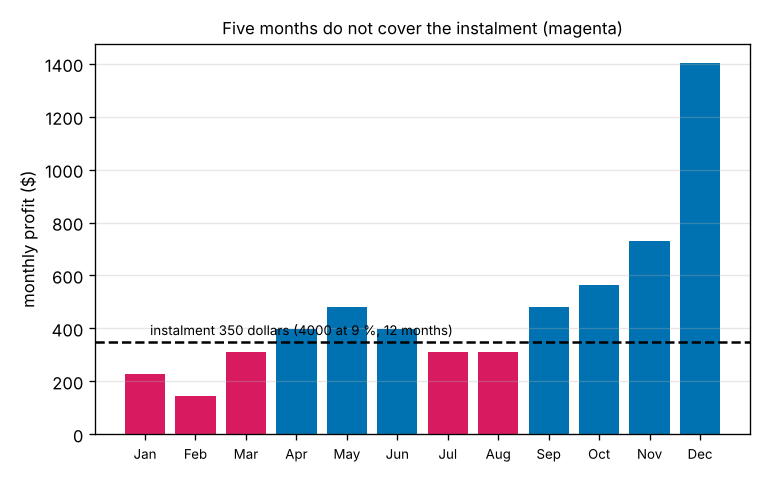
\includegraphics[width=0.95\linewidth]{figures/s05_monthly_profit.png}\\\small The twelve monthly profits against the instalment of a 4000 dollar, 12-month loan; the months that do not cover it are magenta.\end{center}

\begin{center}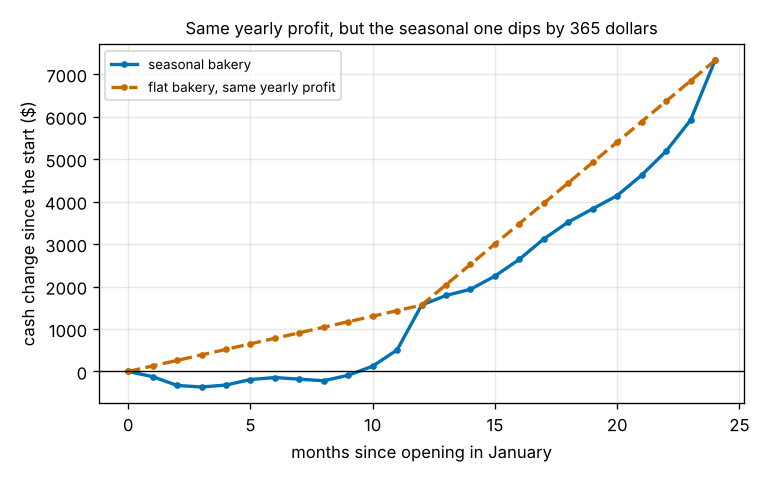
\includegraphics[width=0.95\linewidth]{figures/s05_cash_dip.png}\\\small Running cash change of the seasonal bakery and of a flat bakery with the same yearly profit; the seasonal one dips 365 dollars below its start in March.\end{center}

\subsection*{E. Worked example}
The bakery borrows 4000 dollars of its 6000 dollar start-up cost at 9 percent a year, repaid over 12 months, and opens in January. Find the instalment, the first month's interest, the running total after January, February and March, and the extra cash the owner needs. Compare with a flat year of the same yearly profit.
\begin{enumerate}[nosep]
\item r = 0.09 / 12 = 0.0075 and A = 4000 x 0.0075 / (1 - 1.0075\textasciicircum{}-12) = 30 / 0.08577 = 349.81 dollars a month. Total repaid 12 x 349.81 = 4197.67, so the interest is 197.67 dollars.
\item The first instalment holds 4000 x 0.0075 = 30.00 dollars of interest and repays 319.81 dollars, leaving a balance of 3680.19.
\item The profits are 228, 144 and 312 dollars, so the cash change is 228 - 349.81 = -121.81 after January, -121.81 + 144 - 349.81 = -327.61 after February and -327.61 + 312 - 349.81 = -365.42 after March. April's profit of 396 brings it up by 46.19, so March is the lowest point.
\item The extra cash needed is 365.42 dollars: the owner starts with 2000 dollars already put in and must find 365 dollars more by March.
\item A flat year earns 480 dollars every month and 480 - 349.81 = 130.19 is positive every month, so the flat bakery needs 0 extra cash. The twelve profits of the seasonal year add up to 5760, the same as 12 x 480; after 12 months both are 5760 - 4197.67 = 1562.33 dollars up.
\end{enumerate}
\textbf{Answer.} The instalment is 349.81 dollars; the running total is -121.81, -327.61 and -365.42 dollars after January to March, so the owner needs 365.42 dollars of extra cash in March; a flat year with the same yearly profit needs none, and both years end 1562.33 dollars ahead. The seasons change when the money arrives, not how much.

\subsection*{F. Questions}
\begin{enumerate}[nosep]
\item \textbf{Conceptual.} A seasonal bakery and a flat bakery earn exactly the same profit over a year. Why can only the seasonal one run short of cash when it repays a loan in equal instalments?
\item \textbf{Numerical.} A loan of 3000 dollars at 12 percent a year is repaid over 12 months. Find the monthly instalment, the interest in the first instalment, the balance after it, and the total interest.
\item \textbf{Graph and simulation interpretation.} In the running-cash figure the seasonal and flat curves are 756 dollars apart in March (-365 against +391) but touch again in December. What does the gap in March mean, and why do the curves meet at month 12?
\item \textbf{Design and optimisation challenge.} Design: the owner borrows 4000 dollars at 9 percent and can find at most 200 dollars of extra cash in the planned year. Choose the shortest loan term among 6, 12, 18 and 24 months that works. What does it cost in interest compared with 12 months, and how risky is it when demand is random?
\end{enumerate}

\section{Real-world mini-project}
\textbf{Choose the price and the oven size for a made-up bakery.} The owner may buy a 600, 800 or 1000 loaf oven (\texttt{OPTIONS} in the Session 3 lesson gives the monthly fixed cost and the start-up cost of each) and may set any price from 3.00 to 5.00 dollars in steps of 0.25. Demand is 1675 minus 250 times the price (loaves per month) and sales cannot exceed the oven's capacity. Use \texttt{evaluate} from Session 3 to report, for every choice, the break-even quantity, the margin of safety, the loss probability and the payback in months. A choice passes if the loss probability is at most 5 percent, the payback is at most 12 months and the margin of safety is at least 20 percent. Among the passing choices, recommend the one with the highest mean monthly profit. General education only: the numbers are made up.

\textbf{The lender's limit on the loss chance.} A lender will fund the bakery if the chance that a month makes a loss is at most 8 percent. The independent model of Session 3 says 9.5 percent, so the plan fails; but price and demand are linked. Use \texttt{loss\_vs\_rho}, \texttt{rho\_for\_limit} and \texttt{implied\_rho} from Session 4 to find which correlations meet the limit, whether the demand line of Session 2 does, and how robust that conclusion is to the seed and to the spread of the price. State clearly that the answer depends on the correlation you assume, and which assumption you would defend to the lender. \textbf{Deliverable:} A script that prints the loss probability for correlations from -0.9 to +0.9 in steps of 0.1, finds the largest correlation that meets the 8 percent limit, reports the correlation implied by the demand line and its loss probability, repeats the calculation for seeds 1 to 5, and saves a plot of the loss probability against the correlation with the limit and the implied value marked. \textbf{Success looks like:} The largest correlation that meets the limit is about -0.19 (loss probability 7.9 percent); the demand line gives -0.33 and a loss probability of 6.9 percent, so it meets the limit, while independent inputs (9.5 percent) and positive correlations (12.4 percent at +0.5) do not; the threshold stays between about -0.20 and -0.14 across seeds 1 to 5.

\textbf{How much should the bakery borrow, and over how long?} The owner can borrow 1000, 2000, 3000, 4000, 5000 or 6000 dollars of the 6000 dollar start-up cost at 9 percent a year, repaid over 6, 12, 18 or 24 months, and opens in January. The owner can find a buffer of 1000 dollars of extra cash. A choice passes if the planned year needs at most 1000 dollars of extra cash and the chance, over 5000 simulated years with random demand, of needing more than 1000 dollars is at most 10 percent. Among the passing choices recommend the one that borrows the most (the owner puts in the least own money), and break ties by the lowest total interest. Use \texttt{evaluate\_loan} and \texttt{loan\_passes} from Session 5. Then say how the answer changes if the bakery opens in October. \textbf{Deliverable:} A script that prints a table of all 24 choices (instalment, total interest, extra cash needed, risk), marks which pass, names the recommended choice, and saves a plot of the extra cash needed against the loan term with one line per loan size. \textbf{Success looks like:} 12 of the 24 choices pass; the recommended choice is 5000 dollars over 24 months (instalment 228.4 dollars, interest 482.2 dollars, 84.8 dollars of extra cash in the planned year and a 7.6 percent chance of needing more than 1000), so the owner puts in only 1000 dollars of own money; 5000 over 18 months (19.0 percent) and 4000 over 12 months (33.0 percent) fail. Opening in October instead, 19 choices pass and the recommended choice becomes 6000 dollars over 18 months, since the strong months now come first.

\section{The path ahead}
\begin{enumerate}[nosep]
\item \textbf{Session 6: Shares of the variance.} A function that reports, for price, variable cost and demand, the share of profit variance it explains.
\item \textbf{Session 7: Design under a risk limit.} A search that adds new oven options and prices, and reports the cheapest design that meets the limit.
\item \textbf{Session 8: A browser lab with live Monte Carlo.} One page with sliders for price, costs, fixed cost and demand, linked to the lines, histogram and tornado chart.
\end{enumerate}

\section{Answers and hints}

\subsection*{Session 1}
\begin{enumerate}[nosep]
\item \textbf{Conceptual.} Hint: Does a cup cost anything to make? Solution: They forgot the variable cost. Each cup brings in 2.00 dollars but also costs 0.50 dollars to make, so it only helps the fixed cost by 1.50 dollars. The right answer is 60 / 1.50 = 40 cups, not 30.
\item \textbf{Numerical.} Hint: Earn per cup = price minus cup cost; then divide. Solution: Each cup earns 1.50 - 0.60 = 0.90 dollars. Cups = 45 / 0.90 = 50. Check: income = 1.50 * 50 = 75 dollars; cost = 45 + 0.60 * 50 = 75 dollars. Equal. Units: dollars divided by dollars per cup gives cups.
\item \textbf{Graph and simulation interpretation.} Hint: Cost line value is 60 plus 0.50 times 25; income is 2.00 times 25. Solution: At 25 cups the cost is 60 + 12.50 = 72.50 dollars and the income is 50 dollars. The profit is 50 - 72.50 = minus 22.50 dollars, a loss: the red line is still above the green line, so the stall is behind.
\item \textbf{Design and optimisation challenge.} Hint: Try price 2.50 with the same fixed cost, and fixed cost 45 with the same price. Then try price 1.00 to see the other direction. Solution: Price 2.50 dollars: each cup earns 2.00, so 60 / 2.00 = 30 cups. Or fixed cost 45 dollars at price 2.00: 45 / 1.50 = 30 cups. Both work. A higher price risks fewer customers (this simple model ignores that); a smaller fixed cost means a cheaper stall, which may be smaller or worse placed. A price of 1.00 dollar would need 60 / 0.50 = 120 cups, so cutting the price a lot pushes break-even far away.
\end{enumerate}

\subsection*{Session 2}
\begin{enumerate}[nosep]
\item \textbf{Conceptual.} Hint: Compute the profit at 720 loaves for each and the percentage drop, or compare the DOL values. Solution: X drops from 480 to 312 dollars, a fall of 35 percent (DOL 3.5). Y has contribution margin 1.35 dollars and profit 1.35 * 720 - 600 = 372 dollars, a fall of 22.5 percent (DOL 2.25). X is riskier because more of its cost is fixed: its profit reacts more strongly to sales. X also gains more in a good month. Operating leverage is risk in both directions.
\item \textbf{Numerical.} Hint: Contribution margin first. Solution: Margin = 5 - 2 = 3 dollars per item. Break-even = 900 / 3 = 300 items and revenue = 300 * 5 = 1500 dollars. For 600 dollars: (900 + 600) / 3 = 500 items. Units: dollars per month divided by dollars per item gives items per month. Sanity check: at 500 items, profit = 3 * 500 - 900 = 600.
\item \textbf{Graph and simulation interpretation.} Hint: The line is (p - v) q - F. Solution: At 0 loaves the profit is minus 1200 dollars: the fixed cost you pay even if you sell nothing. The slope is 2.10 dollars per loaf, the contribution margin. The line crosses zero at 571.43 loaves, the break-even. To the right of it you are in profit.
\item \textbf{Design and optimisation challenge.} Hint: Solve 250 p\textasciicircum{}2 - 2025 p + 4045 = 0, or scan prices on a grid and look for profit = 500. Solution: Two prices work: about 3.58 and 4.52 dollars. At 3.58 the bakery sells about 780 loaves, at 4.52 about 545. Both have margin of safety 500 / 1700 = 29.4 percent, but the cheaper price needs more flour, labour and oven time and has the larger break-even (551 loaves against 384). The most profit is at 4.05 dollars, about 555.6 dollars, so a target of 600 dollars cannot be reached at any price. Trade-off: the higher price gives the same profit with less work but depends on the demand estimate being right.
\end{enumerate}

\subsection*{Session 3}
\begin{enumerate}[nosep]
\item \textbf{Conceptual.} Hint: Think of the weighted contribution margin and the sales mix. Solution: The break-even units are F divided by the weighted margin. If the mix shifts towards the product with the larger margin per unit (cakes, 9.00 dollars, against 2.10 for loaves), the weighted margin rises and the break-even falls: 430.1 units for 90 percent loaves, 344.8 for 80 percent and 246.9 for 60 percent. The fixed cost and prices did not change; only the mix did.
\item \textbf{Numerical.} Hint: Monthly rate = 1.12\textasciicircum{}(1/12) - 1. Add up discounted cash month by month and compare with 6000. Solution: Simple payback: 6000 / 480 = 12.5 months, so the running total first reaches zero in month 13. The monthly rate is 0.9489 percent. Discounted payback is month 14. The 24 month NPV is 4259 dollars (5520 dollars with no discounting). Discounting lowers the value of later cash, so the discounted payback is later and the NPV smaller. Units: dollars and months.
\item \textbf{Graph and simulation interpretation.} Hint: Look at the area left of the zero line, and at how the width changes. Solution: The loss probability is the share of the area (about 9.5 percent of the 20000 months) to the left of zero, the red part. A larger demand standard deviation widens the histogram. The mean profit stays near 480 dollars (the simulated mean is 476) but more months fall below zero, so the loss probability rises.
\item \textbf{Design and optimisation challenge.} Hint: Loop over capacity and price, print loss, payback and mean profit, and filter with \texttt{passes}. Solution: Only the 600 loaf oven at 4.00 and 4.25 dollars passes. The best of them for profit is 4.25 dollars: break-even about 351 loaves, average sales about 546, margin of safety about 36 percent, loss probability about 4 percent, mean profit about 556 dollars a month and payback 9 months. A price of 3.50 fails because the payback is 21 months, and the 1000 loaf oven does not pay back within 36 months at 4.00 dollars because demand is below its capacity most months, so its extra fixed cost is wasted. Trade-off: the biggest oven looks safest for growth but has the highest fixed cost; the small oven loses some sales when demand is high.
\end{enumerate}

\subsection*{Session 4}
\begin{enumerate}[nosep]
\item \textbf{Conceptual.} Hint: Think about what a month with a higher price than planned does to the margin and to the number of loaves sold. Solution: Profit is the margin per loaf times the number of loaves. A month with a high price has a bigger margin but, with a negative correlation, a smaller demand; a month with a low price has a smaller margin but a bigger demand. The two effects pull the profit in opposite directions and partly cancel, so the profit varies less around the same centre: this is a natural hedge. The average moves only by rho sigma\_p sigma\_D (here 15 dollars at -0.5) while the standard deviation falls from 375 to 301 dollars, so fewer months fall below zero. With a positive correlation the effects add and the risk grows.
\item \textbf{Numerical.} Hint: Cov = rho sigma\_p sigma\_D = 15. Use the variance formula and then z = -mean / standard deviation. Solution: Mean = 480 + 15 = 495 dollars. Variance = 99 225 + 40 000 + 2 x 2.1 x 800 x 15 + 1 406 + 225 = 99 225 + 40 000 + 50 400 + 1 406 + 225 = 191 256, so the standard deviation is 437.3 dollars. z = -495 / 437.3 = -1.132 and P(loss) = 0.129, about 12.9 percent, a little above the simulated 12.4 percent. The shortcut is slightly high at both +0.5 and -0.5 because of the skew. Units: dollars per month, and a pure number for the probability.
\item \textbf{Graph and simulation interpretation.} Hint: Where does the curve cross 8 percent, and what does the demand-line value assume about why price moves? Solution: The curve crosses 8 percent at a correlation of about -0.19, so any correlation below that meets the limit. The demand line implies -0.33, which meets it with 6.9 percent. What we cannot conclude is that the plan is safe: the -0.33 holds only if the price wobbles because the bakery moves along its demand line, so that 50 of the 150 loaves of demand spread are explained by price. If the price wobbles for other reasons (a supplier's cost, a competitor's sale) the link may be weaker, and at a correlation of 0 the limit is missed. The result depends on an assumption about the cause of the price changes and should be reported as a range (6.9 to 9.5 percent), not as one number.
\item \textbf{Design and optimisation challenge.} Hint: Use \texttt{loss\_probability(rho, fixed=...)} for F = 1200, 1150, 1100, 1050 and 1000. Solution: Independent inputs: 1200 gives 9.5 percent, 1150 gives 7.0, 1100 gives 5.1 (just over) and 1050 gives 3.6, so the highest fixed cost that meets the limit is 1050 dollars. With the correlation -0.33: 1200 gives 6.9 percent, 1150 gives 4.9 and 1100 gives 3.5, so the highest is 1150 dollars. Believing the correlation relaxes the budget by 100 dollars a month. But 4.9 percent is only 0.1 points below the limit, within the error of the simulation (about 0.2 points for 20000 months), and it rests on the assumed correlation; a careful owner who cannot rule out independent inputs would choose 1050 dollars, which meets the limit under both assumptions (3.6 and 2.4 percent). The constants are made-up, so this shows a method, not a real loan decision.
\end{enumerate}

\subsection*{Session 5}
\begin{enumerate}[nosep]
\item \textbf{Conceptual.} Hint: Compare each month's profit with the instalment, and think about when the money arrives. Solution: The instalment is the same in every month, but the seasonal bakery earns its profit unevenly: in the five quiet months (January, February, March, July and August) the profit is below the 349.81 dollar instalment, so the cash falls, and the strong months (above all December) come later. The running total is the sum of the monthly gains and losses, so it can go below its start in March and climb back later, even though the yearly total is the same as for the flat bakery, whose 480 dollar profit covers the instalment every month. The seasons change when the money arrives, not how much, and cash is needed at the time the bill is due.
\item \textbf{Numerical.} Hint: r = 0.12 / 12 = 0.01 and A = L r / (1 - (1 + r)\textasciicircum{}-n). Solution: r = 0.01. A = 3000 x 0.01 / (1 - 1.01\textasciicircum{}-12) = 30 / 0.11255 = 266.55 dollars. The first month's interest is 3000 x 0.01 = 30.00 dollars, so 266.55 - 30.00 = 236.55 dollars is repaid and the balance is 3000 - 236.55 = 2763.45 dollars. Total paid 12 x 266.55 = 3198.56, so the total interest is 198.56 dollars. Units: dollars (and dollars a month for the instalment).
\item \textbf{Graph and simulation interpretation.} Hint: What do the two bakeries have in common after twelve months, and what differs in March? Solution: After twelve months both bakeries have earned 5760 dollars and paid the same twelve instalments, so both are 1562 dollars up: the curves meet. Both have paid three instalments (1049 dollars), but by March the flat bakery has earned 3 x 480 = 1440 dollars of profit and the seasonal one only 684 dollars. That is 756 dollars less, so the seasonal line sits 756 dollars below the flat one (-365 against +391). The 756 dollars is not lost: the seasonal bakery earns it back in the strong months from October to December. Until then the owner has to bridge the part of it that takes the total below the start, the 365 dollars of extra cash.
\item \textbf{Design and optimisation challenge.} Hint: Use \texttt{extra\_cash\_needed} for each term, then \texttt{total\_interest} and \texttt{shortfall\_probability(1000, loan=4000, term=...)}. Solution: The extra cash needed is 2150 dollars for 6 months, 365 for 12, 105 for 18 and 0 for 24. The shortest term with at most 200 dollars is 18 months (105 dollars). Its interest is 291.0 dollars against 197.7 dollars for 12 months, an extra 93.3 dollars for the smaller instalment (238.39 against 349.81). With random demand the chance of needing more than 1000 dollars is 8.7 percent for 18 months (33.0 percent for 12 months and 4.3 percent for 24). The 18-month loan meets the rule, but only just: with the owner's 200 dollar buffer a bad winter would need more, so a careful owner might accept the extra interest of 24 months (385.7 dollars) or open in April, when even the 12-month loan needs no extra cash. The numbers are made up, so this shows a method, not a lending decision.
\end{enumerate}

\section{How to join}
Read \texttt{CONTRIBUTING.md} in the repository, then pick an issue labelled \texttt{good first issue}. Repository: \url{https://github.com/KrunalPanchal1995/pan-iit-oss/tree/main/openbreakeven}

\end{document}
